\subsection{Aufbauorganisation}
Die Aufbauorganisation bestimmt welche Aufgaben von welchen Personen übernommen werden. Sie grenzt sich von der Ablauforganisation ab, welche den Ablauf von Leistungs- und Produktionsprozessen bestimmt. Um eine Aufbauorganisation darzustellen bieten sich Leitungssysteme an, welche speziell Führungs- und Entscheidungsprozesse im Unternehmen organisieren. Die grafische Darstellung eines Leitungssystem ist z.B. das sog. Organigramm, welches zusätzlich Abteilungen oder Teams darstellen kann.

Leistungssysteme lassen sich folgendermaßen differenzieren:

\begin{table}[H]
    \centering
    \begin{tabularx}{\textwidth}{|c|X|X|X|X|}
        \hline
                   & Einliniensystem                                                                                                                                          & Stab-Liniensystem                                                                                                                 & Mehrliniensystem (Funktional)                                                                                                                                                                                                                             & Matrixsystem                                                                                                                                                                                                                                                        \\
        \hline
        Grundsatz  & Eine untergeordnete Stelle erhält jeweils nur von einer vorgesetzten Instanz Anweisungen. Die Linie bildet gleichzeitig den kommunikativen Dienstweg ab. & Ein um Stäbe erweitertes Einliniensystem. Die Stäbe haben keine Weisungsbefugnis sondern bereiten Entscheidungen vor und beraten. & Spezialisten sind für definierte Funktionen zuständig und unmittelbar fachlich weisungsbefugt. Anforderungen bzw. Anweisungen können von verschiedenen Vorgesetzten kommen und Instanzen auf gleicher Ebene können unmittelbar miteinander kommunizieren. & Es existieren zwei weitestgehend unabhängige Hierarchien o. Dimensionen. Z.B. können Funktionen und Objekte oder Projekte sein. An Kreuzungspunkten befinden sich fachliche Spezialisten, welche Anforderungen von überall bekommen können, aber meist autark sind. \\
        \hline
        Schema     & siehe Abb. \ref{fig:einliniensystem}                                                                                                                     & siehe Abb. \ref{fig:stabliniensystem}                                                                                             & siehe Abb. \ref{fig:mehrliniensystem}                                                                                                                                                                                                                     & siehe Abb. \ref{fig:matrixsystem}                                                                                                                                                                                                                                   \\
        \hline
        Eigenarten & Streng hierarchisches Denken und große Macht bei Leitungskräften.                                                                                        & Trennung von Entscheidungs- und Fachkompetenz.                                                                                    & Spezialisierung der Instanzen und verkürzte Delegations- und Informationswege.                                                                                                                                                                            & Autarke und schnell agierende Instanzen.                                                                                                                                                                                                                            \\
        \hline
        Vorteile   & klare Zuständigkeiten, einfach, Konflikte wg. widersprüchlichen Anweisungen unwahrscheinlich                                                             & Entlastung der Führungskräfte, Trennung und Konzentration Entscheidungs- und Fachkompetenzen                                      & höhere Flexibilität, schnellere Entscheidungsfindung, Entlastung durch Spezialisierung der Führungskräfte                                                                                                                                                 & optimierte Ressourcennutzung, Flexibilität und Dynamik, Förderung interdisziplinärer Zusammenarbeit                                                                                                                                                                 \\
        \hline
        Nachteile  & hohe Last bei Führungskräften, geringe Flexibilität, lange Kommunikationswege                                                                            & mögliche unklare Verantwortungen, Konfliktmöglichkeit zwischen Führungskraft und Stab                                             & hohes Konfliktpotential zwischen Führungskräften, unklare Verantwortlichkeiten, Komplexität                                                                                                                                                               & Konfliktpotential zwischen Führungskräften, Komplexität insbesondere der Kommunikation und Koordination, Hoher Abstimmungsaufwand für die Gesamtunternehmensplanung                                                                                                 \\
        \hline
    \end{tabularx}
    \caption{Leitungssysteme}
    \label{tab:leitungssysteme}
\end{table}


\begin{figure}[H]
    \centering
    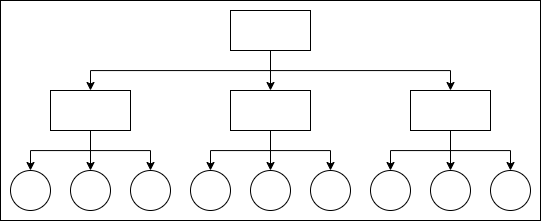
\includegraphics[width=\textwidth]{figures/einliniensystem.png}
    \caption{Einliniensystem}
    \label{fig:einliniensystem}
\end{figure}
\FloatBarrier

\begin{figure}[H]
    \centering
    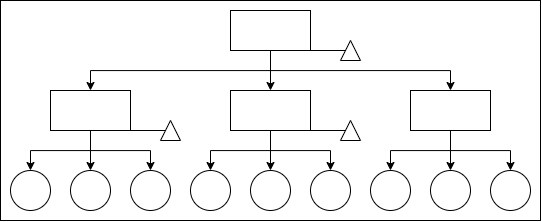
\includegraphics[width=\textwidth]{figures/stabliniensystem.png}
    \caption{Stab-Liniensystem}
    \label{fig:stabliniensystem}
\end{figure}
\FloatBarrier

\begin{figure}[H]
    \centering
    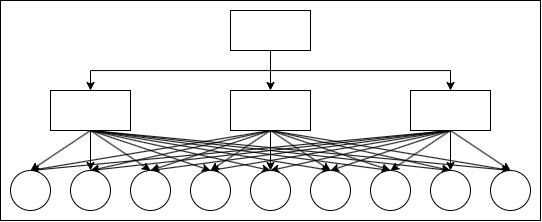
\includegraphics[width=\textwidth]{figures/mehrliniensystem.png}
    \caption{Mehrliniensystem}
    \label{fig:mehrliniensystem}
\end{figure}
\FloatBarrier

\begin{figure}[H]
    \centering
    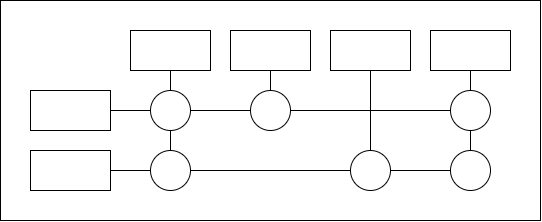
\includegraphics[width=\textwidth]{figures/matrixsystem.png}
    \caption{Matrixsystem}
    \label{fig:matrixsystem}
\end{figure}
\FloatBarrier